\begin{frame}{}

  \vspace{1cm}
  \begin{figure}\centering
    \definecolor{c1}{rgb}{0 0.4470 0.7410}
\definecolor{c2}{rgb}{0.8500 0.3250 0.0980}
\definecolor{c3}{rgb}{0.9290 0.6940 0.1250}
\definecolor{c4}{rgb}{0.4940 0.1840 0.5560}
\definecolor{c5}{rgb}{0.4660 0.6740 0.1880}
\definecolor{c6}{rgb}{0.3010 0.7450 0.9330}
\definecolor{c7}{RGB}{251,180,185}
\definecolor{c8}{RGB}{247,104,161}
\definecolor{c9}{RGB}{255,0,255}

% GNUPLOT: LaTeX picture with Postscript
\begingroup
  \makeatletter
  \providecommand\color[2][]{%
    \GenericError{(gnuplot) \space\space\space\@spaces}{%
      Package color not loaded in conjunction with
      terminal option `colourtext'%
    }{See the gnuplot documentation for explanation.%
    }{Either use 'blacktext' in gnuplot or load the package
      color.sty in LaTeX.}%
    \renewcommand\color[2][]{}%
  }%
  \providecommand\includegraphics[2][]{%
    \GenericError{(gnuplot) \space\space\space\@spaces}{%
      Package graphicx or graphics not loaded%
    }{See the gnuplot documentation for explanation.%
    }{The gnuplot epslatex terminal needs graphicx.sty or graphics.sty.}%
    \renewcommand\includegraphics[2][]{}%
  }%
  \providecommand\rotatebox[2]{#2}%
  \@ifundefined{ifGPcolor}{%
    \newif\ifGPcolor
    \GPcolorfalse
  }{}%
  \@ifundefined{ifGPblacktext}{%
    \newif\ifGPblacktext
    \GPblacktexttrue
  }{}%
  % define a \g@addto@macro without @ in the name:
  \let\gplgaddtomacro\g@addto@macro
  % define empty templates for all commands taking text:
  \gdef\gplfronttext{}%
  \gdef\gplfronttext{}%
  \makeatother
  \ifGPblacktext
    % no textcolor at all
    \def\colorrgb#1{}%
    \def\colorgray#1{}%
  \else
    % gray or color?
    \ifGPcolor
      \def\colorrgb#1{\color[rgb]{#1}}%
      \def\colorgray#1{\color[gray]{#1}}%
      \expandafter\def\csname LTw\endcsname{\color{white}}%
      \expandafter\def\csname LTb\endcsname{\color{black}}%
      \expandafter\def\csname LTa\endcsname{\color{black}}%
      \expandafter\def\csname LT0\endcsname{\color[rgb]{1,0,0}}%
      \expandafter\def\csname LT1\endcsname{\color[rgb]{0,1,0}}%
      \expandafter\def\csname LT2\endcsname{\color[rgb]{0,0,1}}%
      \expandafter\def\csname LT3\endcsname{\color[rgb]{1,0,1}}%
      \expandafter\def\csname LT4\endcsname{\color[rgb]{0,1,1}}%
      \expandafter\def\csname LT5\endcsname{\color[rgb]{1,1,0}}%
      \expandafter\def\csname LT6\endcsname{\color[rgb]{0,0,0}}%
      \expandafter\def\csname LT7\endcsname{\color[rgb]{1,0.3,0}}%
      \expandafter\def\csname LT8\endcsname{\color[rgb]{0.5,0.5,0.5}}%
    \else
      % gray
      \def\colorrgb#1{\color{black}}%
      \def\colorgray#1{\color[gray]{#1}}%
      \expandafter\def\csname LTw\endcsname{\color{white}}%
      \expandafter\def\csname LTb\endcsname{\color{black}}%
      \expandafter\def\csname LTa\endcsname{\color{black}}%
      \expandafter\def\csname LT0\endcsname{\color{black}}%
      \expandafter\def\csname LT1\endcsname{\color{black}}%
      \expandafter\def\csname LT2\endcsname{\color{black}}%
      \expandafter\def\csname LT3\endcsname{\color{black}}%
      \expandafter\def\csname LT4\endcsname{\color{black}}%
      \expandafter\def\csname LT5\endcsname{\color{black}}%
      \expandafter\def\csname LT6\endcsname{\color{black}}%
      \expandafter\def\csname LT7\endcsname{\color{black}}%
      \expandafter\def\csname LT8\endcsname{\color{black}}%
    \fi
  \fi
    \setlength{\unitlength}{0.0500bp}%
    \ifx\gptboxheight\undefined%
      \newlength{\gptboxheight}%
      \newlength{\gptboxwidth}%
      \newsavebox{\gptboxtext}%
    \fi%
    \setlength{\fboxrule}{0.5pt}%
    \setlength{\fboxsep}{1pt}%
\begin{picture}(8000.00,4800.00)%
    \gplgaddtomacro\gplfronttext{%
      \colorrgb{0.15,0.15,0.15}%
      \put(-52,2909){\makebox(0,0)[r]{\strut{}\small $80\%$}}%
      \colorrgb{0.15,0.15,0.15}%
      \put(-52,3369){\makebox(0,0)[r]{\strut{}\small $85\%$}}%
      \colorrgb{0.15,0.15,0.15}%
      \put(-52,3830){\makebox(0,0)[r]{\strut{}\small $90\%$}}%
      \colorrgb{0.15,0.15,0.15}%
      \put(-52,4290){\makebox(0,0)[r]{\strut{}\small $95\%$}}%
      \colorrgb{0.15,0.15,0.15}%
      \put(-52,4751){\makebox(0,0)[r]{\strut{}\small $100\%$}}%
      \colorrgb{0.15,0.15,0.15}%
      \put(1583,2228){\makebox(0,0){\strut{}}}%
      \colorrgb{0.15,0.15,0.15}%
      \put(562,2228){\makebox(0,0){\strut{}}}%
      \colorrgb{0.15,0.15,0.15}%
      \put(324,2228){\makebox(0,0){\strut{}}}%
      \colorrgb{0.15,0.15,0.15}%
      \put(86,2228){\makebox(0,0){\strut{}}}%
    }%
    \gplgaddtomacro\gplfronttext{%
      \colorrgb{0.15,0.15,0.15}%
      \put(-718,3599){\rotatebox{90}{\makebox(0,0){\strut{}$\sigma_{\bm{M}} = 0.0$ m}}}%
      \colorrgb{0.00,0.00,0.00}%
      \put(831,4971){\makebox(0,0){\strut{}$\sigma_R = 0.01$ m}}
      \put(3999,5900){\makebox(0,0){\strut{}Ποσοστό επιτυχίας στόχου (\ref{objective:02_04}) ανά μονάδα αρχικής μετατόπισης $|\Delta\theta|$}}%
      \put(0,5400){\makebox(0,0){\strut{}{\color{c1}{\rule[0.6mm]{0.5cm}{0.5mm}}}\small PLICP}}
      \put(1000,5400){\makebox(0,0){\strut{}{\color{c2}{\rule[0.6mm]{0.5cm}{0.5mm}}}\small NDT}}
      \put(2000,5400){\makebox(0,0){\strut{}{\color{c3}{\rule[0.6mm]{0.5cm}{0.5mm}}}\small FastGICP}}
      \put(3400,5400){\makebox(0,0){\strut{}{\color{c4}{\rule[0.6mm]{0.5cm}{0.5mm}}}\small FastVGICP}}
      \put(4800,5400){\makebox(0,0){\strut{}{\color{c5}{\rule[0.6mm]{0.5cm}{0.5mm}}}\small NDT-PSO}}
      \put(6100,5400){\makebox(0,0){\strut{}{\color{c6}{\rule[0.6mm]{0.5cm}{0.5mm}}}\small TEASER}}
      \put(7000,5400){\makebox(0,0){\strut{}{\color{c7}{\rule[0.6mm]{0.5cm}{0.5mm}}}\small x1}}
      \put(7600,5400){\makebox(0,0){\strut{}{\color{c8}{\rule[0.6mm]{0.5cm}{0.5mm}}}\small uf}}
      \put(8200,5400){\makebox(0,0){\strut{}{\color{c9}{\rule[0.6mm]{0.5cm}{0.5mm}}}\small fm}}
      \put(3999,-550){\makebox(0,0){\strut{}Αρχική μετατόπιση $|\Delta \theta|$ [rad]}}%
    }
    \gplgaddtomacro\gplfronttext{
      \colorrgb{0.15,0.15,0.15}
      \put(1532,2448){\makebox(0,0)[r]{\strut{}}}
      \colorrgb{0.15,0.15,0.15}%
      \put(1532,2909){\makebox(0,0)[r]{\strut{}}}%
      \colorrgb{0.15,0.15,0.15}%
      \put(1532,3369){\makebox(0,0)[r]{\strut{}}}%
      \colorrgb{0.15,0.15,0.15}%
      \put(1532,3830){\makebox(0,0)[r]{\strut{}}}%
      \colorrgb{0.15,0.15,0.15}%
      \put(1532,4290){\makebox(0,0)[r]{\strut{}}}%
      \colorrgb{0.15,0.15,0.15}%
      \put(1532,4751){\makebox(0,0)[r]{\strut{}}}%
      \colorrgb{0.15,0.15,0.15}%
      \put(3167,2228){\makebox(0,0){\strut{}}}%
      \colorrgb{0.15,0.15,0.15}%
      \put(2146,2228){\makebox(0,0){\strut{}}}%
      \colorrgb{0.15,0.15,0.15}%
      \put(1908,2228){\makebox(0,0){\strut{}}}%
      \colorrgb{0.15,0.15,0.15}%
      \put(1670,2228){\makebox(0,0){\strut{}}}%
    }%
    \gplgaddtomacro\gplfronttext{%
      \colorrgb{0.00,0.00,0.00}%
      \put(2415,4971){\makebox(0,0){\strut{}$\sigma_R = 0.03$ m}}%
    }%
    \gplgaddtomacro\gplfronttext{%
      \colorrgb{0.15,0.15,0.15}%
      \put(3116,2448){\makebox(0,0)[r]{\strut{}}}%
      \colorrgb{0.15,0.15,0.15}%
      \put(3116,2909){\makebox(0,0)[r]{\strut{}}}%
      \colorrgb{0.15,0.15,0.15}%
      \put(3116,3369){\makebox(0,0)[r]{\strut{}}}%
      \colorrgb{0.15,0.15,0.15}%
      \put(3116,3830){\makebox(0,0)[r]{\strut{}}}%
      \colorrgb{0.15,0.15,0.15}%
      \put(3116,4290){\makebox(0,0)[r]{\strut{}}}%
      \colorrgb{0.15,0.15,0.15}%
      \put(3116,4751){\makebox(0,0)[r]{\strut{}}}%
      \colorrgb{0.15,0.15,0.15}%
      \put(4751,2228){\makebox(0,0){\strut{}}}%
      \colorrgb{0.15,0.15,0.15}%
      \put(3730,2228){\makebox(0,0){\strut{}}}%
      \colorrgb{0.15,0.15,0.15}%
      \put(3492,2228){\makebox(0,0){\strut{}}}%
      \colorrgb{0.15,0.15,0.15}%
      \put(3254,2228){\makebox(0,0){\strut{}}}%
    }%
    \gplgaddtomacro\gplfronttext{%
      \colorrgb{0.00,0.00,0.00}%
      \put(3999,4971){\makebox(0,0){\strut{}$\sigma_R = 0.05$ m}}%
    }%
    \gplgaddtomacro\gplfronttext{%
      \colorrgb{0.15,0.15,0.15}%
      \put(4700,2448){\makebox(0,0)[r]{\strut{}}}%
      \colorrgb{0.15,0.15,0.15}%
      \put(4700,2909){\makebox(0,0)[r]{\strut{}}}%
      \colorrgb{0.15,0.15,0.15}%
      \put(4700,3369){\makebox(0,0)[r]{\strut{}}}%
      \colorrgb{0.15,0.15,0.15}%
      \put(4700,3830){\makebox(0,0)[r]{\strut{}}}%
      \colorrgb{0.15,0.15,0.15}%
      \put(4700,4290){\makebox(0,0)[r]{\strut{}}}%
      \colorrgb{0.15,0.15,0.15}%
      \put(4700,4751){\makebox(0,0)[r]{\strut{}}}%
      \colorrgb{0.15,0.15,0.15}%
      \put(6335,2228){\makebox(0,0){\strut{}}}%
      \colorrgb{0.15,0.15,0.15}%
      \put(5314,2228){\makebox(0,0){\strut{}}}%
      \colorrgb{0.15,0.15,0.15}%
      \put(5076,2228){\makebox(0,0){\strut{}}}%
      \colorrgb{0.15,0.15,0.15}%
      \put(4838,2228){\makebox(0,0){\strut{}}}%
    }%
    \gplgaddtomacro\gplfronttext{%
      \colorrgb{0.00,0.00,0.00}%
      \put(5583,4971){\makebox(0,0){\strut{}$\sigma_R = 0.10$ m}}%
    }%
    \gplgaddtomacro\gplfronttext{%
      \colorrgb{0.15,0.15,0.15}%
      \put(6284,2448){\makebox(0,0)[r]{\strut{}}}%
      \colorrgb{0.15,0.15,0.15}%
      \put(6284,2909){\makebox(0,0)[r]{\strut{}}}%
      \colorrgb{0.15,0.15,0.15}%
      \put(6284,3369){\makebox(0,0)[r]{\strut{}}}%
      \colorrgb{0.15,0.15,0.15}%
      \put(6284,3830){\makebox(0,0)[r]{\strut{}}}%
      \colorrgb{0.15,0.15,0.15}%
      \put(6284,4290){\makebox(0,0)[r]{\strut{}}}%
      \colorrgb{0.15,0.15,0.15}%
      \put(6284,4751){\makebox(0,0)[r]{\strut{}}}%
      \colorrgb{0.15,0.15,0.15}%
      \put(7919,2228){\makebox(0,0){\strut{}}}%
      \colorrgb{0.15,0.15,0.15}%
      \put(6898,2228){\makebox(0,0){\strut{}}}%
      \colorrgb{0.15,0.15,0.15}%
      \put(6660,2228){\makebox(0,0){\strut{}}}%
      \colorrgb{0.15,0.15,0.15}%
      \put(6422,2228){\makebox(0,0){\strut{}}}%
    }%
    \gplgaddtomacro\gplfronttext{%
      \colorrgb{0.00,0.00,0.00}%
      \put(7167,4971){\makebox(0,0){\strut{}$\sigma_R = 0.20$ m}}%
    }%
    \gplgaddtomacro\gplfronttext{%
      \colorrgb{0.15,0.15,0.15}%
      \put(-52,509){\makebox(0,0)[r]{\strut{}\small $80\%$}}%
      \colorrgb{0.15,0.15,0.15}%
      \put(-52,969){\makebox(0,0)[r]{\strut{}\small $85\%$}}%
      \colorrgb{0.15,0.15,0.15}%
      \put(-52,1430){\makebox(0,0)[r]{\strut{}\small $90\%$}}%
      \colorrgb{0.15,0.15,0.15}%
      \put(-52,1890){\makebox(0,0)[r]{\strut{}\small $95\%$}}%
      \colorrgb{0.15,0.15,0.15}%
      \put(-52,2351){\makebox(0,0)[r]{\strut{}\small $100\%$}}%
      \colorrgb{0.15,0.15,0.15}%
      \put(1583,-172){\makebox(0,0){\strut{}\small $\frac{\pi}{4}$}}%
      \colorrgb{0.15,0.15,0.15}%
      \put(562,-172){\makebox(0,0){\strut{}\small $\frac{\pi}{8}$}}%
      \colorrgb{0.15,0.15,0.15}%
      \put(324,-172){\makebox(0,0){\strut{}\small $\frac{\pi}{16}$}}%
      \colorrgb{0.15,0.15,0.15}%
      \put(86,-172){\makebox(0,0){\strut{}\footnotesize $0.0$}}%
    }%
    \gplgaddtomacro\gplfronttext{%
      \colorrgb{0.15,0.15,0.15}%
      \put(-718,1199){\rotatebox{90}{\makebox(0,0){\strut{}$\sigma_{\bm{M}} = 0.05$ m}}}%
    }%
    \gplgaddtomacro\gplfronttext{%
      \colorrgb{0.15,0.15,0.15}%
      \put(1532,48){\makebox(0,0)[r]{\strut{}}}%
      \colorrgb{0.15,0.15,0.15}%
      \put(1532,509){\makebox(0,0)[r]{\strut{}}}%
      \colorrgb{0.15,0.15,0.15}%
      \put(1532,969){\makebox(0,0)[r]{\strut{}}}%
      \colorrgb{0.15,0.15,0.15}%
      \put(1532,1430){\makebox(0,0)[r]{\strut{}}}%
      \colorrgb{0.15,0.15,0.15}%
      \put(1532,1890){\makebox(0,0)[r]{\strut{}}}%
      \colorrgb{0.15,0.15,0.15}%
      \put(1532,2351){\makebox(0,0)[r]{\strut{}}}%
      \colorrgb{0.15,0.15,0.15}%
      \put(3167,-172){\makebox(0,0){\strut{}\small $\frac{\pi}{4}$}}%
      \colorrgb{0.15,0.15,0.15}%
      \put(2146,-172){\makebox(0,0){\strut{}\small $\frac{\pi}{8}$}}%
      \colorrgb{0.15,0.15,0.15}%
      \put(1908,-172){\makebox(0,0){\strut{}\small $\frac{\pi}{16}$}}%
      \colorrgb{0.15,0.15,0.15}%
      %\put(1670,-172){\makebox(0,0){\strut{}\footnotesize $0.0$}}%
    }%
    \gplgaddtomacro\gplfronttext{%
    }%
    \gplgaddtomacro\gplfronttext{%
      \colorrgb{0.15,0.15,0.15}%
      \put(3116,48){\makebox(0,0)[r]{\strut{}}}%
      \colorrgb{0.15,0.15,0.15}%
      \put(3116,509){\makebox(0,0)[r]{\strut{}}}%
      \colorrgb{0.15,0.15,0.15}%
      \put(3116,969){\makebox(0,0)[r]{\strut{}}}%
      \colorrgb{0.15,0.15,0.15}%
      \put(3116,1430){\makebox(0,0)[r]{\strut{}}}%
      \colorrgb{0.15,0.15,0.15}%
      \put(3116,1890){\makebox(0,0)[r]{\strut{}}}%
      \colorrgb{0.15,0.15,0.15}%
      \put(3116,2351){\makebox(0,0)[r]{\strut{}}}%
      \colorrgb{0.15,0.15,0.15}%
      \put(4751,-172){\makebox(0,0){\strut{}\small $\frac{\pi}{4}$}}%
      \colorrgb{0.15,0.15,0.15}%
      \put(3730,-172){\makebox(0,0){\strut{}\small $\frac{\pi}{8}$}}%
      \colorrgb{0.15,0.15,0.15}%
      \put(3492,-172){\makebox(0,0){\strut{}\small $\frac{\pi}{16}$}}%
      \colorrgb{0.15,0.15,0.15}%
      %\put(3254,-172){\makebox(0,0){\strut{}\footnotesize $0.0$}}%
    }%
    \gplgaddtomacro\gplfronttext{%
    }%
    \gplgaddtomacro\gplfronttext{%
      \colorrgb{0.15,0.15,0.15}%
      \put(4700,48){\makebox(0,0)[r]{\strut{}}}%
      \colorrgb{0.15,0.15,0.15}%
      \put(4700,509){\makebox(0,0)[r]{\strut{}}}%
      \colorrgb{0.15,0.15,0.15}%
      \put(4700,969){\makebox(0,0)[r]{\strut{}}}%
      \colorrgb{0.15,0.15,0.15}%
      \put(4700,1430){\makebox(0,0)[r]{\strut{}}}%
      \colorrgb{0.15,0.15,0.15}%
      \put(4700,1890){\makebox(0,0)[r]{\strut{}}}%
      \colorrgb{0.15,0.15,0.15}%
      \put(4700,2351){\makebox(0,0)[r]{\strut{}}}%
      \colorrgb{0.15,0.15,0.15}%
      \put(6335,-172){\makebox(0,0){\strut{}\small $\frac{\pi}{4}$}}%
      \colorrgb{0.15,0.15,0.15}%
      \put(5314,-172){\makebox(0,0){\strut{}\small $\frac{\pi}{8}$}}%
      \colorrgb{0.15,0.15,0.15}%
      \put(5076,-172){\makebox(0,0){\strut{}\small $\frac{\pi}{16}$}}%
      \colorrgb{0.15,0.15,0.15}%
      %\put(4838,-172){\makebox(0,0){\strut{}\footnotesize $0.0$}}%
    }%
    \gplgaddtomacro\gplfronttext{%
    }%
    \gplgaddtomacro\gplfronttext{%
      \colorrgb{0.15,0.15,0.15}%
      \put(6284,48){\makebox(0,0)[r]{\strut{}}}%
      \colorrgb{0.15,0.15,0.15}%
      \put(6284,509){\makebox(0,0)[r]{\strut{}}}%
      \colorrgb{0.15,0.15,0.15}%
      \put(6284,969){\makebox(0,0)[r]{\strut{}}}%
      \colorrgb{0.15,0.15,0.15}%
      \put(6284,1430){\makebox(0,0)[r]{\strut{}}}%
      \colorrgb{0.15,0.15,0.15}%
      \put(6284,1890){\makebox(0,0)[r]{\strut{}}}%
      \colorrgb{0.15,0.15,0.15}%
      \put(6284,2351){\makebox(0,0)[r]{\strut{}}}%
      \colorrgb{0.15,0.15,0.15}%
      \put(7919,-172){\makebox(0,0){\strut{}\small $\frac{\pi}{4}$}}%
      \colorrgb{0.15,0.15,0.15}%
      \put(6898,-172){\makebox(0,0){\strut{}\small $\frac{\pi}{8}$}}%
      \colorrgb{0.15,0.15,0.15}%
      \put(6660,-172){\makebox(0,0){\strut{}\small $\frac{\pi}{16}$}}%
      \colorrgb{0.15,0.15,0.15}%
      %\put(6422,-172){\makebox(0,0){\strut{}\footnotesize $0.0$}}%
    }%
    \gplgaddtomacro\gplfronttext{%
    }%
    \put(0,0){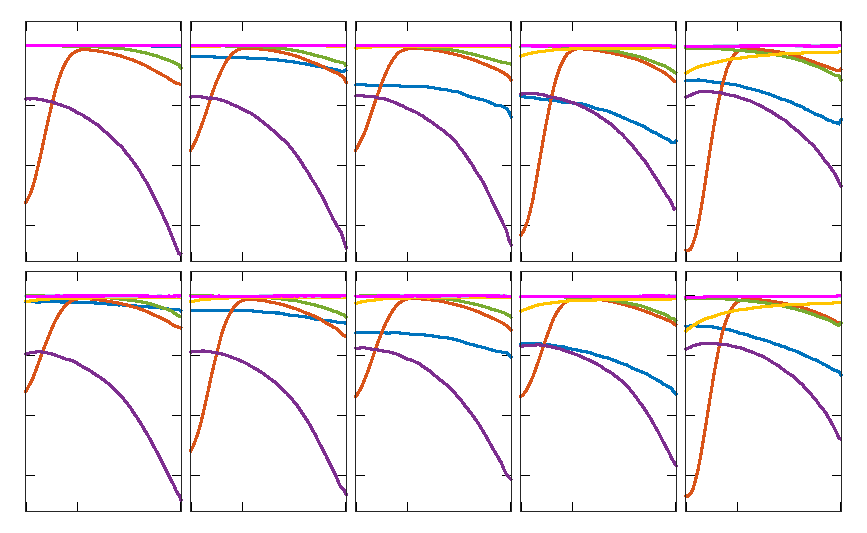
\includegraphics{./figures/parts/02/chapters/04/sections/05/orientation_improvement_percent_binned_curves}}%
    \gplfronttext
  \end{picture}%
\endgroup

  \end{figure}


\note{\footnotesize
Αυτό λοιπόν που είνα σήμερα δυνατόν που δεν ηταν προηγουμένως είναι η ύπαρξη
  \textbf{τριών} μεθόδων που λύνουν το πρόβλημα sm2 χωρίς να χρησιμοποιούν
  αντιστοιχίσεις, οι οποίες είναι περισσότερο ακριβείς και εύρωστες από εκείνες
  της βιβλιογραφίας που εκτελούνται σε πραγματικό χρόνο. Έπειτα οποιαδήποτε από
  αυτές τις τρεις μεθόδους είναι ικανή να λύσει και το πρόβλημα της παρατήρησης
  της στάσης ενός οχήματος καθώς αυτό κινείται, και το πρόβλημα της εκτίμησης
  της στάσης του εκ του μηδενός, χωρίς να χρησιμοποιούνται πουθενά ad hoc
  μεταβλητές ή features.}

\end{frame}
